\chapter[Models]{Methods}

This work utilized both linear and nonlinear methods for analysis, modeling, and prediction, including Auto-Regressive Moving Average models with eXogenous inputs (ARMAX) and neural net models. No single method is ideal, and using many methods is better for insight, especially for nonlinear/complex systems. The details of their application will be expanded upon in their respective sections.

\section{Linear}

\subsection{Overview}
Due to its simplicity and ease of application, linear models are used in practically all fields as a first attempt to interpret data and any potential relationships. In Space Physics, where the underlying behavior of a complex system is not theoretically known, and in-situ measurements are sparse, linear models are often the first step towards understanding what components are related and to what degree. Sometimes this leads to understanding unexpected complexities in a system.


\subsection{ARX}

Impulse response systems are systems in which the output (a response) is driven by a linear sum of coefficients of an input (a series of impulses). A simple example would be making a loud noise in a concert hall. The response will be the unique echoes and reverberations created by the initial driving sound, and with enough signal, a statistical model can be generated that will map the input sound to a response echo. In the magnetosphere, the most used example is an impulse of $v_{B_S}$ driving the Auroral Electrojet (AE/AL) index \citep{VBzAL}, or the Disturbance Storm Time ($D_{st}$) index \citep{VBzDST}. $v_{B_S}$ is a metric where solar wind velocity is multiplied by the southward component of the solar wind magnetic field (i.e. southward components keep their value, northward components are zeroed). This model is  shown in Figure \ref{VBzIRplot}

\begin{figure}[htp]
\centering
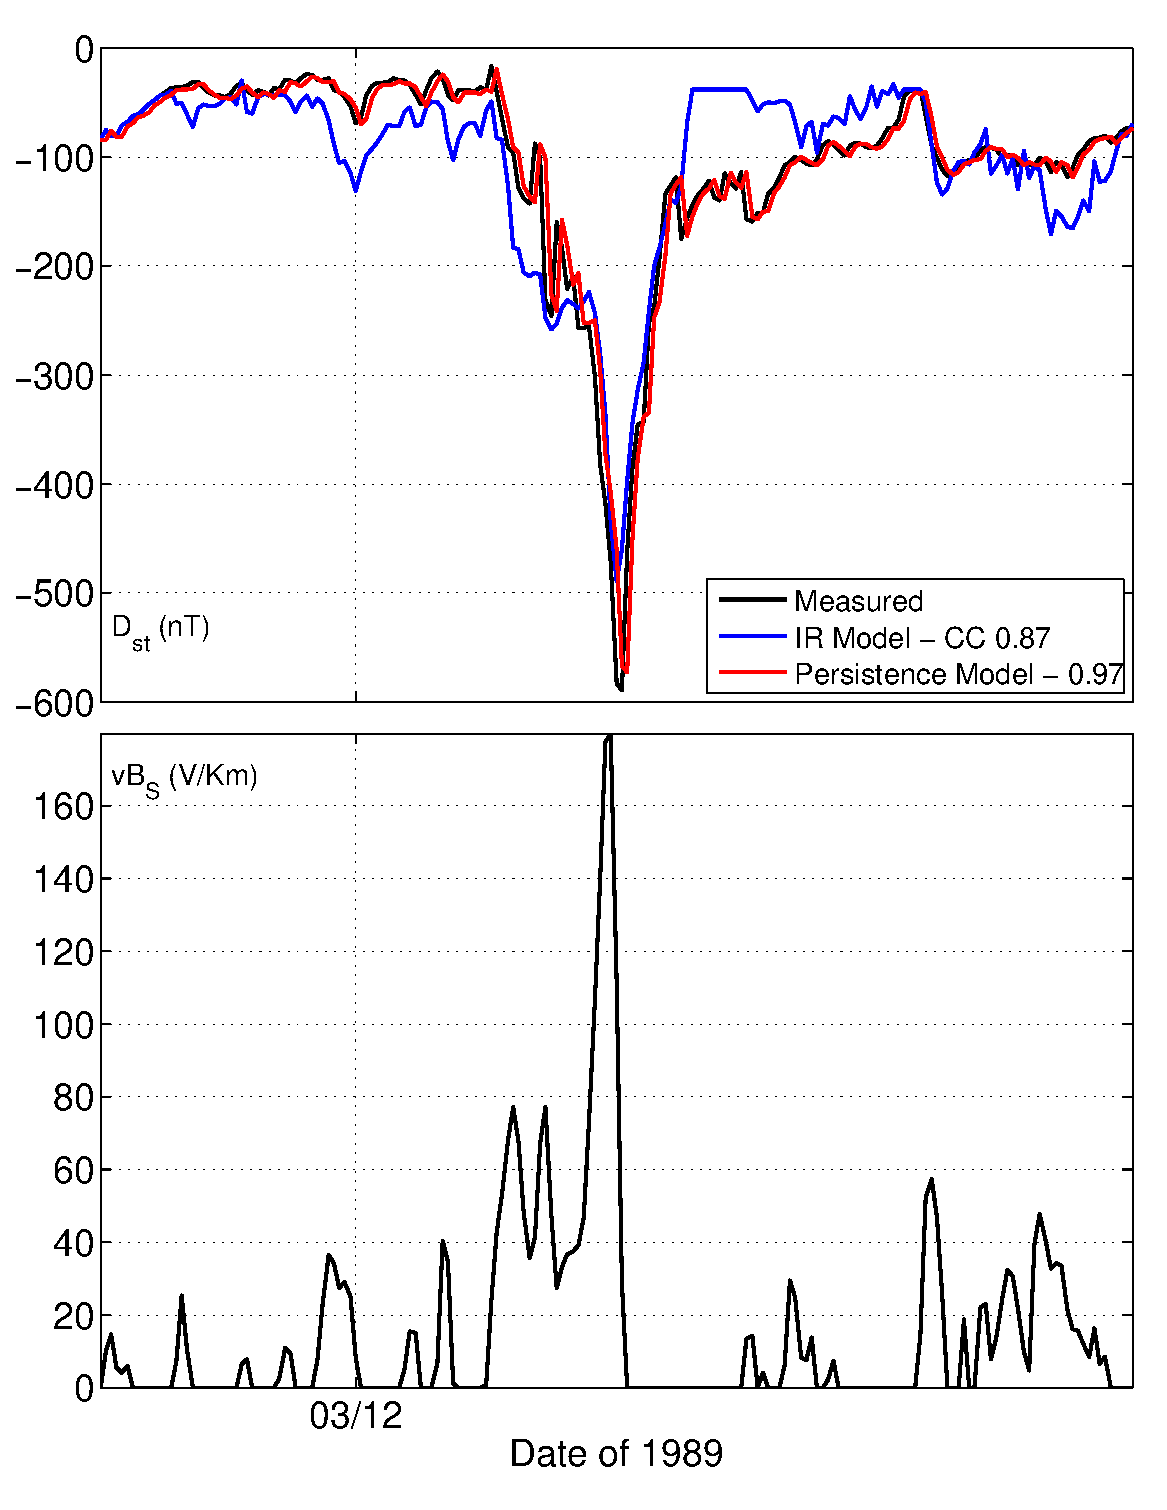
\includegraphics[scale=0.40]{{Figures/BasicModelExample-GOES6}}
\caption{(a) \dst\ (black), persistence (red), 12-hour impulse response model (blue). (b) $v_{B_S}$ impulse as input.}
\label{VBzIRplot}
\end{figure}

This plot shows how different models are used to predict magnetospheric variables with varying amounts of success. In this proposal, what starts as a Box-Jenkins model of the form \citep{DOYvar}:
\begin{align*}
x(t)&=\sum_{j=1}^{m}{b_j \cdot f(t-j\Delta t)}+c_t
\end{align*}
can be modified to include an auto-regressive component to be an autoregressive model with exogenous inputs (ARX) such as that used in \cite{ARXEqn}, taking the form:
\begin{align}
\hat{x}(t)&=\sum_{i=1}^la_i\cdot x(t-i\Delta t)+\sum_{j=1}^m b_j\cdot f(t-j\Delta t)+c_t
\label{ARXEqn}
\end{align}
Where $m$ and $l$ are the number of coefficients desired for including previous data points in the prediction, and $c$ is a factor to remove the mean offset from the data. Note that in some cases the starting value of the iterators can be individually increased if there is a known delay in response time or there is a desire to predict further into the future. In \cite{ARXEqn}, second order equations ($m=2$) were used with anywhere from one to four driving coefficients, but in practice any number of coefficients and any number of driving variables can be used up to some fraction of the number of data points that allows the coefficient matrices to be solved for. 

There generally is a limit to the usefulness of large-lead-time forecasts \cite{ExtremeEvents}. By looking at a plot of the cross correlation relative to the number of coefficients, a limit will generally be seen where adding more coefficients no longer reduces error in the model. By creating a threshhold of change in fit per coefficient added (perhaps via a bootstrap method), the minimum number of coefficients needed to optimally model the system can be determined.

By constructing a linear system of equations from Equation \ref{ARXEqn}, the coefficients can be solved for in a general matrix form (where, in this case, $l=m$):
\[
\left( \begin{array}{ccccccc}
x_0 & ... & x_{l-1} & f_0 & ... & f_{l-1} & 1\\
x_1 &     & x_l & f_l &  &f_l & 1\\
... &     &     &     &  &   & \\
x_{N-l} & ... & x_{N-1} & f_{N-l} & ... & f_{N-1} & 1
\end{array} \right)
\left(\begin{array}{c}
a_0\\...\\a_{l-1}\\b_0\\...\\b_{l-1}\\c
\end{array}\right)
=
\left(
\begin{array}{c}
x_l \\ x_{l+1} \\ ... \\ x_{N}
\end{array}
\right)
\]

This is a linear model for the behavior of a system. However, it has been shown that the set of coefficients describing the response of a system can change with storm intensity \cite{ARXEqn}, the time scale modeled \cite{Coupling}, and even the time of day \cite{VBzAL}. This creates a very large number of possible directions for research, from predicting storm onsets, to predicting storm intensities, to modeling the overall shape and behavior of a storm, as well as all of the other possible interactions outside of storm-time. 


\subsection{ARMAX}

A class of model known as an Auto-Regressive Moving Average with eXogenous inputs model (ARMAX) is often used in time series analysis to combine the effects of persistence, linear dependence, and an average that changes with time. It makes a slight change on the ARX model in Equation \ref{ARXEqn}, adding the moving average term:

\begin{align}
\hat{x}(t)&=\sum_{i=1}^la_i\cdot x(t-i\Delta t)+\sum_{j=1}^m b_j\cdot f(t-j\Delta t)+\sum_{k=1}^n e_j\cdot c(t-k\Delta t)+c_t
\label{ARMAXEqn}
\end{align}


\subsection{Applicability}
As implied by the name, an ARMAX model is suitable for analysis of a time-dependent linear system where the value of a measurement is determined by its own persistence, an external variable, and some factor that contributes to a moving average with time. Most linear systems can be encapsulated by this framework, some even being overspecified with this level of accounting for variability.

\subsection{Caveats and Biases}
There will be a number of things that, ideally, must come together to make this kind of data prediction work. For one: ARX methods can often be heavily dependent on a concept known as ``persistence", whereby the best prediction for a variable at any time is that same variable at the last measured time step. For example, if the high temperature today is $70^\circ$, it is fairly likely that the high temperature tomorrow will be near $70^\circ$. Too much reliance on persistence forecasting, though, and predictions can lose their usefulness. Figure \ref{VBzIRplot}, for example, shows how a model can achieve high correlation with persistence, but be almost entirely useless for predicting events before they happen since the spikes are never anticipated, just modeled after they've already been seen. Also, if the time of interest is multiple time-steps ahead, a simple persistence forecast becomes less and less accurate with each step.

In this case, it is clear that the most recent measurement has the most weight in a forecast. For day-to-day behavior, this is acceptable as being part of the behavior of the system. For the forecasting of extreme events, however, another metric must be used that measures the ability of the model to predict events at or before their actual occurrence, while simultaneously avoiding predicting events that do not happen. One method for comparing models in this fashion is by using the Heidke Skill Score \cite{Heidke,Brier}, which is based on the quantity:
\begin{align*}
S=\frac{R-E}{T-E}
\end{align*}

\note Drop this part if not actually used 

where $R$ is the number of correct forecasts, $T$ is the total number of forecasts, and $E$ is the number expected to be correct by, in this case, a persistence forecast. This can be adapted to either consider a range of "correctness", or a binary threshold to be met. It may also be desired to assign a cost-weighting to success rates. If, say, it costs \$1 million to prepare a power grid for a storm, 10 false alarms to every one storm gets costly unless successfully preparing for that one storm saves \$1 billion. To do this, a measure of the utility of a forecast can be quantified \cite{WeigelDecision}:
\begin{align*}
U_F\equiv BN_H-CN_{\bar{H}}>0
\end{align*}
Where $N_H$ is the number of correct forecasts, $N_{\bar{H}}$ is the number of false alarms, $C$ is the cost of taking mitigating action, and $B$ is the benefit from correctly taking mitigating action. This method has caveats discussed in \cite{WeigelDecision}, but is a useful metric for forecast utility when costs are known, and some measure of success can be determined. 

The other major problem in forecasting is that of lead time. Being able to forecast a storm one minute in advance is generally not enough time for operators to take mitigating action.

\begin{figure}[h!]
	\centering
	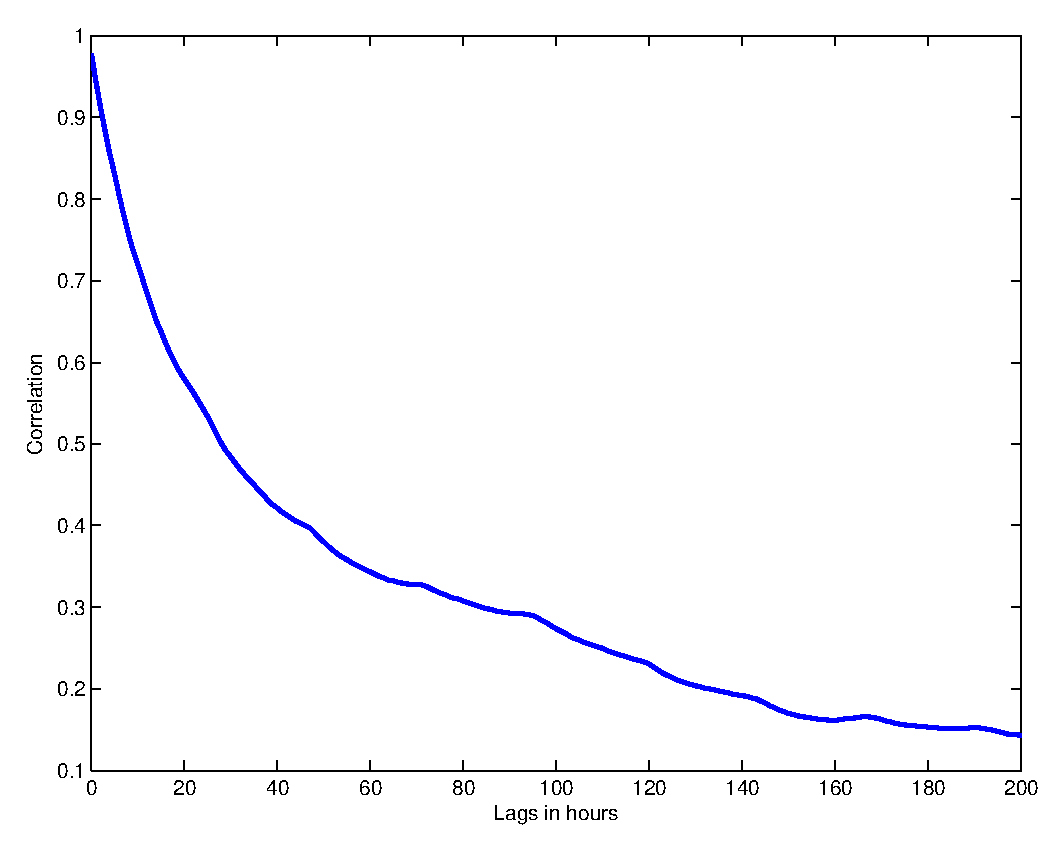
\includegraphics[scale=0.50]{{Figures/PersistentCorrelation.eps}}
	\caption{Correlation between prediction and measurement vs lead time of forecast}
	\label{Lags}
\end{figure}

Figure \ref{Lags} shows the correlation of a set of predictions made for autocorrelation in the disturbance storm time index (\dst) against the amount of lead time in the forecasts. This metric is a measure of how much disturbances in the magnetosphere induce currents in ground-based electrical systems. The predictions were made further and further in time from the current magnetic field and \dst\ measurements, with decreasing accuracy as the predicted time got further from the current time. While an accurate prediction can be made one hour in advance, a prediction 3 days in advance has almost no correlation with what was measured. This is one of the main problems that this dissertation hopes to address.

\subsubsection{Mean vs Median}
The question of whether to use means or medians for analysis is based on what facets of the data are most important to the research. Since means are biased towards outliers and medians biased against them \inote{cite}, the decision rests on how much weight should be given to outliers (or extreme values) in a study. For example, when looking at long-term solar wind variables, intermittent spikes may not be relevant to the overall pattern of behavior being analyzed, but knowing that on a short time scale a certain day had a noticeable spike may be important. In the former case, using the median would likely be best, and using the mean for the latter. However, space physics often deals with skewed distributions and sparse data, leading to an uncertainty of which method is best, so both are and analyzed with their respective traits in mind.
\note Numerically specific result. E.g. 27 day F10.7 vs \req\ with medians vs means

\subsubsection{Effects of time averaging}
Similarly to the mean vs median question, the decision on if/how much to average the data over time will affect the resulting time series to be biased against intermittent spikes in value. The more time added to any particular average, the less impact any short-term changes will have on the final value.

\subsection{Summary}
Because linear models are simple, optimizable, and adequately model many physical systems, they are a useful first choice for trying to determine the behavior of mass density in the plasmatrough. The relationships between solar wind, plasmatrough, and plasmasphere may also be detectable on the first order approximation by a linear model if not entirely linear in nature.


\section{Nonlinear}

\subsection{Overview}

While many nonlinear systems are approximated by a number of localized linear models for the sake of simplicity and ease of interpretation, the design and implementation of nonlinear models has become greatly simplified in recent years. Their use allows for determining nonlinear structure without pre-assuming any localization of the data, and as such were used to attempt forecasting in this dissertation. The first choice was a model based on neural networks \citep{NNARMA,ANNforecast} which approximates a non-linear system given a set of training data. The usefulness of this is apparent in a few key points: the weights of contribution of any particular variable to a system will likely be nonlinear in some fashion (e.g. a ground station's measurements will depend on sunlight heating the ionosphere which depends on latitude, time of year, and time of day), and allowing for the non-linear effects of saturation where perhaps the magnetosphere will behave differently after reaching certain levels of particle density or electric potential, rather than directly scaling regardless of limits.

Another algorithm known as Principal Component Analysis (PCA) can be used to take the large number of possible variables and define an orthogonal set of vectors that most efficiently encapsulate the variance in the data. By doing this, the number of variables needed for computing any linear or non-linear algorithm can be reduced and optimized, making predictions quicker while maintaining most of the predictive benefits of using all possible data, as well as indicating which variables contain the most information relevant to the predictions.


\subsection{Neural Networks}

\subsection{Applicability}
Nonlinear models are applicable when a system has more complexity than can be encapsulated by a linear model. Since they're usually a class of model that trains adaptive weights that can be tuned by known inputs and outputs, they're especially useful for systems where a large amount of training data are available.

\subsection{Caveats and Biases}
Nonlinear models can be susceptible to overfitting, since they inherently attempt to fit more complexity than a linear model, but can also be controlled via the number of inputs and weights used. They also may suggest more structure than might truly exist. Both of these problems are lessened by training with more data, if available. Figure \ref{NNvsLinear} shows a comparison of predicting equatorial mass density (\req) with the $F_{10.7}$ index and the disturbance storm time index (\dst). The neural net models (left)  shows much more structure than the linear models (right) despite being given the same data. Whether that structure reflects any real physical phenomenon, however, is a difficult problem to answer, and so both models are often compared to attempt to ascertain what structure may be valid. 

Sometimes, as in the top two plots of Figure \ref{NNvsLinear}, the structure seems to support the same conclusion where the nonlinear model just adds slight detail. Othertimes, as in the case of the lower two plots, the results seem discrepant. The linear model indicates increasing \req\ with increasing $B_z$ and increasing \f, while the nonlinear model shows a more nuanced structure with increased \req\ showing up with lower $B_z$ values, and at a range of \f\ values. Situations like these require further analysis to determine the true underlying structure.

\begin{figure}[h!]
	\centering
	\includegraphics[scale=0.35]{Figures/{NNDst-F107-rhoeq-GOES6}.eps}
		\includegraphics[scale=0.35]{Figures/{LinearDst-F107-rhoeq-GOES6}.eps}
			\includegraphics[scale=0.35]{Figures/{NNBz-F107-rhoeq-GOES5}.eps}
			\includegraphics[scale=0.35]{Figures/{LinearBz-F107-rhoeq-GOES5}.eps}
	\caption{Nonlinear models (left) vs linear models (right) of $\rho_{eq}$}
	\label{NNvsLinear}
\end{figure}


\subsection{Comparison to Linear Model}
Nonlinear models differ from linear models by incorporating some method for accounting for effects within a domain that are not seen across the entire domain. Though both models can be given the same inputs, and trained on the same outputs, the models themselves can fundamentally differ. Linear models are also generally simple to interpret (e.g. $y=2*x$ means for every change in $x$, $y$ changes by double that amount.) Nonlinear models, on the other hand, often have no simple interpretation and must be approached by testing for a range of parameters in the model to map out resulting outputs and make some interpretation of the underlying structure.

Nonlinear models can be compared to a linear model of the same data in order to assess the usefulness of accounting for nonlinear features. If both models result in similar correlation values, it can be said that the nonlinear model offers no extra insight into the structure of the system and the relationships therein. 

\subsection{Summary}
Nonlinear models are a useful addition to linear models by allowing for better approximations to more complex physical systems, where the entire system may not fit a linear model or may have localized dependencies. 



